\documentclass[10pt,conference,a4paper]{IEEEtran_EDM}
\IEEEoverridecommandlockouts
% The preceding line is only needed to identify funding in the first footnote. If that is unneeded, please comment it out.
\usepackage{cite}
\usepackage{amsmath,amssymb,amsfonts}
\usepackage{algorithmic}
\usepackage{graphicx}
\usepackage{textcomp}
\usepackage{xcolor}
\usepackage{listings}
\def\BibTeX{{\rm B\kern-.05em{\sc i\kern-.025em b}\kern-.08em
    T\kern-.1667em\lower.7ex\hbox{E}\kern-.125emX}}

\def\confheader{}

\makeatletter
\newcommand{\linebreakand}{%
  \end{@IEEEauthorhalign}
  \hfill\mbox{}\par
  \mbox{}\hfill\begin{@IEEEauthorhalign}
}
\makeatother

\usepackage{flushend} % <------------- used for automatically balance the columns on the last page. Be careful, read HOWTO XIV. LAST PAGE COLUMN EQUALIZATION

\lstdefinelanguage{JavaScript}{
    keywords={typeof, new, true, false, catch, function, return, null, catch, switch, var, if, in, while, do, else, case, break},
    keywordstyle=\color{blue}\bfseries,
    ndkeywords={class, export, boolean, throw, implements, import, this},
    ndkeywordstyle=\color{darkgray}\bfseries,
    identifierstyle=\color{black},
    sensitive=false,
    comment=[l]{//},
    morecomment=[s]{/*}{*/},
    commentstyle=\color{purple}\ttfamily,
    stringstyle=\color{red}\ttfamily,
    morestring=[b]',
    morestring=[b]"
}

\lstdefinelanguage{Solidity}{
    keywords={typeof, new, true, false, catch, function, return, null, catch, switch, var, if, in, while, do, else, case, break, contract, public, private, view, returns, memory, mapping, address, string, push},
    keywordstyle=\color{blue}\bfseries,
    ndkeywords={class, export, boolean, throw, implements, import, this},
    ndkeywordstyle=\color{darkgray}\bfseries,
    identifierstyle=\color{black},
    sensitive=false,
    comment=[l]{//},
    morecomment=[s]{/*}{*/},
    commentstyle=\color{purple}\ttfamily,
    stringstyle=\color{red}\ttfamily,
    morestring=[b]',
    morestring=[b]"
}


\begin{document}

\markboth{\confheader}{}
\title{Data storage in a decentralized network}

\author{
\IEEEauthorblockN{Dinar D. Khayrutdinov}
\IEEEauthorblockA{\textit{Automated management}\\
\textit{systems department}\\
\textit{National University of Oil and Gas}\\
\textit{"Gubkin University"}\\
Moscow, Russian Federation \\
khayrutdinov.dd@gmail.com}
\and
\IEEEauthorblockN{Denis A. Volkov}
\IEEEauthorblockA{\textit{Automated management}\\
\textit{systems department}\\
\textit{National University of Oil and Gas}\\
\textit{"Gubkin University"}\\
Moscow, Russian Federation \\
denis@volkov.top}
\and
\IEEEauthorblockN{Anastasia G. Mukhina}
\IEEEauthorblockA{\textit{Automated management}\\
\textit{systems department}\\
\textit{National University of Oil and Gas}\\
\textit{"Gubkin University"}\\
Moscow, Russian Federation \\
me@anastasiag.ru}
\and
}

\maketitle


\begin{abstract}
The paper focuses on a decentralized model of storing information in the educational field, as well as its advantages and disadvantages.
Close attention is paid to security, accessibility and confidentiality.
In addition to discussing decentralized networks from a functionality perspective, the article also describes the process of implementing distributed networks in government agencies such as universities for the purpose of persistent and secure data storage.
A comparison is made of classical database management systems with distributed file storage systems such as IPFS.
A description of the architecture of a decentralized application is given, which allows simple direct user interaction with file storage through a convenient and intuitive interface.
A smart contract is considered as a link between the application and the blockchain, ensuring speed, transparency and reliability of the transaction.
A decentralized application, smart contracts and an interface for information output have been developed.
It is concluded that decentralized data storage is an innovation that has every chance of becoming an important component of Web3.

\end{abstract}

\begin{IEEEkeywords}
Decentralization, blockchain, smart contract, security, decentralized applications, distributed file systems, privacy, encryption.
\end{IEEEkeywords}

\section{Introduction}
% This document is a model and instructions for \LaTeX.
% Please observe the conference page limits. 
Today, information technology is developing at an exorbitant pace as never before.
Human life is shrouded in all kinds of technology amenities that provide easy and fast interaction with the services offered.
It is difficult to imagine a person who does not use social networks, a bank application and other digital innovations.
In addition to the notable advantages of these technologies, there is another side that is associated with data leaks, hacks and hacker attacks.
Information protection is one of the main goals of modern companies that face various problems when storing data on local devices.
In this regard the use of decentralized storage has become the most suitable option to meet the needs of businesses in data storage and management.
If you follow the standards of the Russian Federation for ensuring information security in organizations \cite{GOST53114}, it becomes possible to secure your data, as well as maintain confidentiality.
The document states that the organization that implements the technology must ensure security, confidentiality and accessibility for the user.
Distributed file systems, blockchain, smart contracts and other decentralized technologies can provide the necessary functionality that will meet the criteria specified in the official document.

The objectives of this work are the analysis of decentralized technologies, the development of necessary services, as well as practical guidance on the implementation of distributed file systems in an organization.

\section{Theory}

\subsection{Description and benefits of using IPFS}

Decentralized storage is a way to store information on multiple nodes connected to a peer–to-peer network (P2P), for example, using BitTorrent or IPFS \cite{IPFS} protocols.
In decentralized networks such as BitTorrent or IPFS, information is broken down into small parts and distributed across different network nodes.
These nodes can be computers of any users connected to the network, which provides additional protection and fault tolerance \cite{Anisimov}.
By storing data on multiple nodes at the same time, even if one or more nodes fail or are attacked, the information remains accessible thanks to other nodes that have copies of the data.

Information uploaded to a storage system that does not have a central node is divided into small parts and distributed across several nodes. If the user wants to access the file, the network collects the separated parts from different nodes and combines them again into a file that can be downloaded. A more illustrative example is shown in Figure \ref{data_IPFS}.

\begin{figure}[htbp]
\centerline{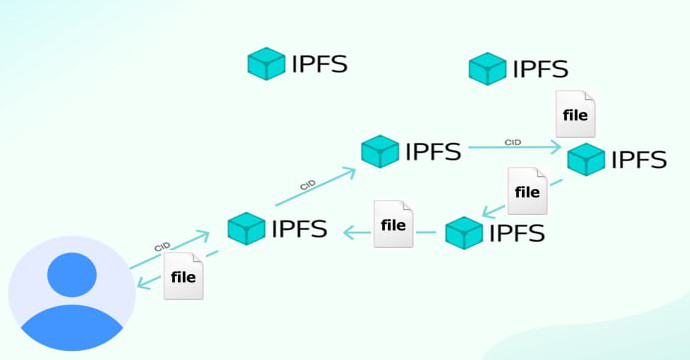
\includegraphics[scale=0.71]{fig1.png}}
\caption{Getting data from IPFS.}
\label{data_IPFS}
\end{figure}

Also, nodes of a decentralized system do not have the ability to view or modify files, since the cryptographic hashing method automatically encrypts all data on the network. To gain access to them, users use their private keys, which protect information from third parties \cite{Web3Browsers}.
Using cloud storage provides significant advantages in data storage, including scalability, simplicity, cost savings, security and flexibility. Users can save their data to cloud storage in any remote location using a dedicated private network connection or the public Internet.

Consider the advantages of storing data in a decentralized network:
\begin{itemize}
    \item \textbf{Fault tolerance}. When one or more nodes fail, data remains available thanks to other nodes in the network.
    \item \textbf{Security}. The use of encryption and other methods ensures data protection in decentralized networks.
    \item \textbf{Efficiency}. Node resources are used more efficiently, as the load is distributed among many participants.
    \item \textbf{Privacy}. Users have more control over their data, as it is not stored in one central location that can be hacked or monitored.
    \item \textbf{Reliability}. Decentralized systems can be more reliable, as they do not depend on a single node or organization.
\end{itemize}
Along with the advantages, there are disadvantages such as:
\begin{itemize}
    \item \textbf{Access}.to information may take longer due to the dependence on the network of nodes.
    \item \textbf{Decentralized}.systems may be vulnerable to malicious nodes, which may pose a threat to data security.
    \item \textbf{Network}.infrastructure problems can also affect data availability.
    \item \textbf{The lack of standartizaion}. In decentralized systems makes it difficult to be compatible between different protocols.
\end{itemize}

\subsection{Decentralized data storage as a Web3 important technology }

Decentralized data storage is a new technology that has not yet been widely adopted, but may become an important element of Web3. Currently, users are looking for more convenient, efficient and secure ways to store information, so platforms with a decentralized structure, such as IPFS, are becoming more and more popular. Due to constant information leaks, rising storage costs and censorship in the traditional space, more and more people are thinking about using decentralized solutions. They can solve some of the problems of centralized analogues, but they also have their drawbacks. Currently, centralized data storage remains a popular choice for many people and will continue to occupy a significant market share, even with the growing demand for decentralized storage.

The complexity of the blockchain topic is due to complex algorithms, specific terms and other technical elements. There is a number of useful literature for those who are just starting their journey in the study of decentralized technologies, with the help of which the essence of the technology and the basic principles of the blockchain become clear \cite{Kube}. In this regard, many organizations, Government Agencies and just ordinary users bypass this technology. For a more detailed immersion into the world of decentralization, it is proposed to introduce a discipline in educational institutions that will cover blockchain technologies from different angles and touch on more complex topics such as cryptography, blockchain platforms and decentralization in general [5]. Thanks to the training centers, there will be specialists who, in turn, will fill in the gaps of ignorance in society.

Many people mistakenly compare the usual DBMS and IPFS. They do perform similar functions, the most important of which is data storage, but they are designed for different purposes [6]. As already mentioned, IPFS is a distributed file system, which means there is no central management. The DBMS, in turn, is designed for processing and managing structured data, usually in JSON format. Most DBMS are presented in the form of relational databases that store data in an organized table with columns and rows [7]. There are also problems with fault tolerance, if the database server broke down for a while, then all transactions that were transmitted at that time may not be saved, fortunately, backup mechanisms are now provided in case of threats to the server, but this does not negate the fact that the DBMS is subject to various failures. 

It happens that direct use of IPFS can make some actions difficult for a user who does not have confident knowledge of distributed networks, which can lead to confusion, as a result of which adverse consequences may occur. To do this, decentralized applications (DApp) were created, with their help, the user does not need to know how and where his data is stored, since a convenient and intuitive interface provides easy use of this platform [8]. In simple terms, a decentralized application serves as a shell between a human and a distributed file system. But in addition to the interface, DApp offers another stage of protection – it is identity verification through the blockchain [9]. The sequence of saving or viewing a file includes user identification, it is assumed that a hash key is stored in the blockchain, with which you can view the file stored in IPFS. The link in this chain is a smart contract. A smart contract is a code that automatically performs the actions prescribed inside the document [10]. A smart contract is valued for its immutability, transparency and reliability. An analogy can be given with a robot that performs its task according to its internal prescribed scenario. A popular programming language for writing smart contracts is Solidity, which runs on the Ethereum blockchain [11]. To fully understand the sequence from verification in a decentralized application to obtaining the desired file, it is proposed to consider in Figure \ref{Sequence}.

\begin{figure}
\centerline{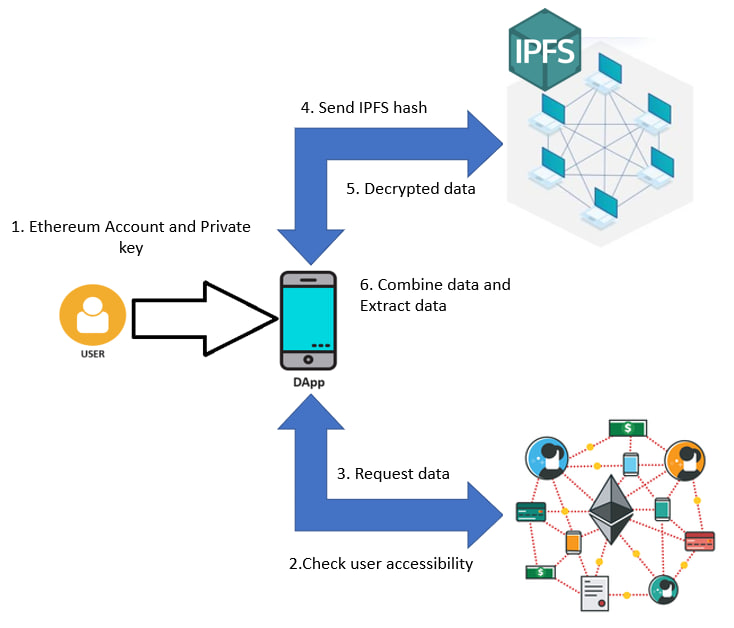
\includegraphics[scale=0.67]{fig2.png}}
\caption{The sequence of operation of decentralized technologies.}
\label{Sequence}
\end{figure}

The first thing a user needs to do is enter their Ethereum account and private key into a decentralized application. Next, with the help of a smart contract, the user is identified on the blockchain side. Upon successful verification, the hash key is returned, which is used to search for the file in IPFS. The final step is to output the desired file to the application interface. 
To implement this technology in a public Institution, it is proposed to follow the following steps [12]:
\begin{itemize}
    \item Assessment of needs and opportunities.
    \item Research and technology selection.
    \item Development of a legal and regulatory framework.
    \item Education and training.
    \item Integration and interaction with existing systems.
    \item System support.
\end{itemize}


\section{Experimental results}
The implementation of a decentralized application that will store the received data in IPFS involves some steps and requires the use of certain tools and libraries. 

First of all, you need to create a DApp server part that will be responsible for receiving, reading and transferring files. Let's use Node.js based on JavaScript [13]. In addition to the basic functionality, you will need to turn to special libraries for working with web3 and IPFS. One of the most popular are Web3.js and js-IPFS. Listing 1 shows one of the main functions that accepts the hash key of a file, invokes a smart contract and stores the transaction in the blockchain.

\lstset{
    language=JavaScript,
    backgroundcolor=\color{white},
    extendedchars=true,
    basicstyle=\scriptsize\ttfamily,
    showstringspaces=false,
    showspaces=false,
    numbers=left,
    numberstyle=\color{white},
    numbersep=9pt,
    tabsize=2,
    breaklines=true,
    showtabs=false,
    captionpos=b
}

\begin{lstlisting}[language=JavaScript, caption=JavaScript code implementing saving to the blockchain]
import Web3 from 'web3';

async function addFileToBlockchain(fileHash) {
    const web3 = new Web3(Web3.givenProvider ||
                          "http://localhost:8545");

    const contractABI = [/* smart contract ABI */];

    const contractAddress = "/*smart contract address*/";

    const contract = new web3.eth.Contract(
                                        contractABI,
                                        contractAddress);

    const accounts = await web3.eth.getAccounts();

    const receipt = await contract.methods.
                        addFile(fileHash).
                            send({ from: accounts[0] });
    return receipt;
}
\end{lstlisting}

To save a file to distributed networks, a function is created that takes the path to the file, initializes IPFS and adds the file that is located at the specified path. After adding, the function returns the hash of the saved file.

\begin{lstlisting}[language=JavaScript, caption= Saving a file to IPFS]
const IPFS = require('ipfs-core');

async function uploadToIPFS(filePath) {
    const jsipfs = await IPFS.create();

    const { cid } = await jsipfs.add(filePath);

    return cid.toString();
}
\end{lstlisting}

After the server part is created, it is proposed to create a smart contract that will link the server written earlier and the blockchain. It is designed to manage and store user hashes. As shown in listing 2, a so-called dictionary is created, which stores data on the principle of key and value. The key is the user's address, and the hash value of the file that is associated with a specific user. In addition to the dictionary, two functions are created, one of which is responsible for adding the transmitted hash file to the user's hash array, and the other provides saved hashes of files associated with the specified user address.

\lstset{
    language=Solidity,
    backgroundcolor=\color{white},
    extendedchars=true,
    basicstyle=\scriptsize\ttfamily,
    showstringspaces=false,
    showspaces=false,
    numbers=left,
    numberstyle=\color{white},
    numbersep=2pt,
    tabsize=2,
    breaklines=true,
    showtabs=false,
    captionpos=b
}

\begin{lstlisting}[caption=Solidity code for a smart contract]
// SPDX-License-Identifier: MIT
pragma solidity ^0.8.0;

contract FileStorage {
    mapping(address => string[]) private userFiles;

    function addFile(string memory fileHash) public {
        userFiles[msg.sender].push(fileHash);
    }

    function getFiles() public view
                        returns (string[] memory) {
        return userFiles[msg.sender];
    }
}
\end{lstlisting}

The React framework is responsible for the interface [14]. This is one of the most popular libraries for the JavaScript programming language, it creates dynamic interfaces, besides it does not require much knowledge in development. The task of the interface is to output information with a valid request, if the server side has caught an error, then the error information should be displayed on the screen. Such situations are not uncommon, exceptions can be either due to a non-existent file or user, or due to breakdowns on the server. The main thing is to handle these errors correctly so that the program does not crash, for this it is necessary to anticipate which exceptions may occur in a given situation.

Thorough testing of all aspects of the program is the key to the stability of the entire system. There are several testing options, for example, for testing and deploying smart contracts, it is proposed to use the Truffle framework, this library has integration with the local Ganache blockchain environment. Simply put, this is a personal local blockchain for testing, with which you can track the transaction of a smart contract. When the server starts, the transaction is saved in a block. Figure \ref{GanacheB} shows the Ganache interface, which displays the user's saved address and balance.

\begin{figure}[htbp]
\centerline{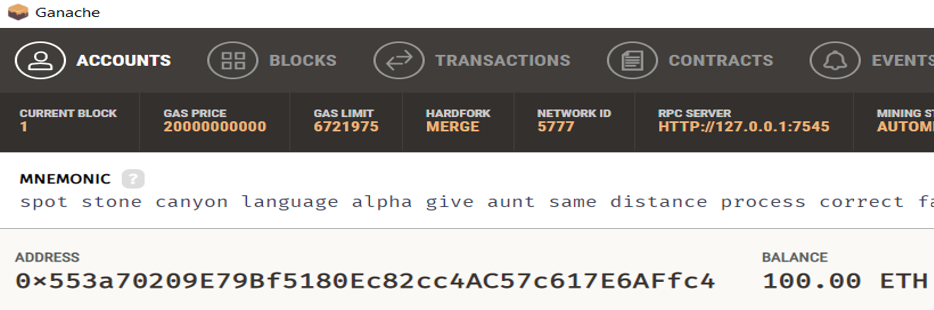
\includegraphics[scale=0.51]{fig3.png}}
\caption{The interface of the local Ganache blockchain.}
\label{GanacheB}
\end{figure}

\section{Conclusions }
In this paper, a decentralized method of storing information in the educational field is considered. The process of implementing distributed networks in Government Institutions is described. DBMS and their differences from IPFS are also considered in detail. Dapp, smart contract, user interface have been developed and all interactions with third-party frameworks have been configured. The application has been tested and has no internal errors.

\begin{thebibliography}{00}

\bibitem{GOST53114} GOST R. 53114–2008 information Protection //Ensuring information security in the organization. Basic terms and definitions. URL: http://docs. cntd. ru/document/1200075565 (accessed: 02.12. 2019)(in Russian). – 2009.

\bibitem{IPFS} InterPlanetary File System. Official website. - https://ipfs.tech/

\bibitem{Anisimov} Maxim Anisimov. Centralized, decentralized and distributed networks: what are they? - https://bytwork.com/articles/vidy-sitey

\bibitem{Web3Browsers} Web3 Browsers for Decentralized Storage. IPFS Blog and News. https://blog.ipfs.tech/2022-01-07-web3-browsers-for-decentralized-storage
\bibitem{Kube} Kube N. Daniel Drescher: Blockchain basics: a non-technical introduction in 25 steps: Apress, 2017, 255 pp, ISBN: 978-1-4842-2603-2. – 2018.
\bibitem{b5} Bashir I. Mastering Blockchain: Deeper insights into decentralization, cryptography, Bitcoin, and popular Blockchain frameworks. – Packt Publishing Limited, 2017.
\bibitem{b6} Ruan P. et al. Blockchains: Decentralized and Verifiable Data Systems. – Springer Nature, 2022.
\bibitem{b7} Gillenson M. L. Fundamentals of database management systems. – John Wiley and Sons, 2023.
\bibitem{b8} Infante R. Building Ethereum Dapps: decentralized applications on the Ethereum blockchain. – Simon and Schuster, 2019.
\bibitem{b9} Lin Iuon-Chang et al. "Symmetry in Blockchain-Powered Secure Decentralized Data Storage: Mitigating Risks and Ensuring Confidentiality" (Symmetry, 2024, Vol. 16, No. 2, Article 147) 
\bibitem{b10} Frolov A.V. Creation of Solidity smart contracts for the Ethereum blockchain //AV Frolov—"LitRes", 2019.-240 p. – 2019.
\bibitem{b11} Khan Nabeel et al. "Proposed Model for Secured Data Storage in Decentralized Cloud by Block-chain Ethereum" (Electronics, 2022, Vol. 11, No. 22, Article 3686)  
\bibitem{b12} Talapina E. V. The use of blockchain in public administration: prospects for legal regulation //Issues of state and municipal management. - 2020. – No. 3. – pp. 96-113
\bibitem{b13} Herron D. Node. js Web Development: Server-side web development made easy with Node 14 using practical examples. – Packt Publishing Ltd, 2020.
\bibitem{b14} Beginning Ethereum and Solidity with React: Complete Guide to becoming a Blockchain Developer Paperback – 7 Jun. 2018 by Greg Lim (Author)
\bibitem{b15} Zheng Zhang, Xiaolian Recovery: A replication protocol using an erasure code in a peer-to-peer storage network. Proceedings of the 21st IEEE Symposium. Reliable Distributed Systems, 2002, pp. 330-335.

\end{thebibliography}


\end{document}
